%% LyX 2.2.1 created this file.  For more info, see http://www.lyx.org/.
%% Do not edit unless you really know what you are doing.
%\documentclass[english]{article}
%\usepackage[latin9]{inputenc}

%\usepackage{babel}
%begin{document}

\documentclass[english]{article}
\usepackage[T1]{fontenc}
\usepackage[latin9]{inputenc}
\usepackage[a4paper]{geometry}
\usepackage{amsmath}
\geometry{verbose,tmargin=2cm,bmargin=2cm,lmargin=2cm,rmargin=2cm}
\usepackage{graphicx}
%\usepackage[chapter]{algorithm}
\usepackage{algorithmic}
\usepackage{tabularx}
\usepackage{colortbl}
\usepackage{hhline}
\newcommand{\norm}[1]{\left\lVert#1\right\rVert}

\DeclareMathOperator*{\argmin}{\arg\!\min}
\DeclareMathOperator*{\argmax}{\arg\!\max}

\makeatletter

%%%%%%%%%%%%%%%%%%%%%%%%%%%%%% LyX specific LaTeX commands.
%% Because html converters don't know tabularnewline
\providecommand{\tabularnewline}{\\}

\makeatother

\usepackage{babel}
\begin{document}

\title{Machine Learning for Computer Vision (EE5177) \\ Programming Assignment 4 : Logistic Regression and SVMs \\ Problem \#1}

\author{Akshit Kumar \\ \emph{EE14B127}}

\date{17th April 2017}

\maketitle
\tableofcontents{}

\section{Introduction}

\subsection{Goal}
The goal of the question is to generate synthetic data of 2 classes of univariate normal distributions with the following parameters:
\begin{itemize}
	\item Class 0 : Mean = -2 , Standard Deviation = 1.5
	\item Class 1 : Mean = 2 , Standard Deviation = 1.5
\end{itemize}
The goal is to find a separating hyperplane for the generated data points for which we use Logistic Regression. The data is not linearly separable which is also evident from the plot. 

\subsection{Approach}
To find the separating hyperplane, during the training phase, we try to minimise the negative log likelihood function. For minimising the log likelihood function and getting the optimal value of $\phi$, we use the \emph{fminunc} MATLAB function which takes in the cost function, the gradient of the cost function and the hessian of the cost function.


\section{Data Generation}
The data is synthesized by randomly sampling from univariate Gaussian distribtuions:
\begin{itemize}
	\item Class 0 : $\mathcal{N}(-2,1.5)$
	\item Class 1 : $\mathcal{N}(2,1.5)$
\end{itemize}
The data is split in the ratio of 80/20 for training and testing respectively.

\section{Training Phase}
\subsection{Goal}
The goal of the training phase is to come up with optimal value of $\phi$ which minimises the negative of the log likelihood function to learn the separating hyperplane.
\subsection{Approach}
The training phase for logistic regression model tries to minimise the negative log likelihood function using the \emph{fminunc} MATLAB function which takes into account the cost function, gradient of the cost function and hessian of the cost function.
The required functions which are passed into the \emph{fminunc} function are :
\begin{itemize}
	\item Cost Function : $L = \Sigma_{i=1}^{I} w_{i}log[\dfrac{1}{1 + \exp(-\phi^Tx_{i})}] + \Sigma_{i=1}^{I} (1-w_{i})log[\dfrac{\exp(-\phi^Tx_{i})}{1 + \exp(-\phi^Tx_{i})}]$ 
	\item Gradient : $\frac{\partial L}{\partial \phi} = -\Sigma_{i=1}^{I} (sig[a_{i}] - w_{i})x_{i}$
	\item Hessian : $\frac{\partial^{2} L}{\partial \phi^2} = -\Sigma_{i=1}^{I} sig[a_{i}](1 - sig[a_{i}])x_{i}x_{i}^T$
\end{itemize}
\subsection{Results}
The optimal values obtained on one trial of the experiment are :(Note : Since the points are sampled randomly, each time we get different optimal points as data changes)
\begin{itemize}
	\item Optimal $\phi$ : $\phi = \begin{bmatrix} 0.31 \\ 2.46 \end{bmatrix}$ 
	\item Gradient at Optimal $\phi$ : $\begin{bmatrix} -8.63e-05 \\ -0.00026 \end{bmatrix}$
	\item Hessian at Optimal $\phi$ : $\begin{bmatrix} 0.0898 & 0.0898 \\ 0.0898 & 0.0898 \end{bmatrix}$
\end{itemize}

\section{Issue with Linear Separability of Data}
When the data is linearly separable, there is an incentive for $\phi$ to get bigger and bigger, to \emph{emphasize} more and more the difference between the two classes. For example, if you double the size of $\phi$, then elements in class 1 get bigger log odds and elements in class 0 get smaller log odds. So from the prespective of minimizing the loss function, it is always better to make $\phi$ bigger and bigger. In this way, $\phi$ won't converge.
One way to deal with the issue is to add regularization to the cost function which penalizes the $\phi$ vector for becoming too large.

\section{Experiment Results}
\subsection{Confusion Matrix}
The confusion matrix obtained is as follows :
$$
\begin{tabularx}{.7\textwidth}{&gt;{\bfseries}c|c c c |}
 & Class 1 & Class 0 \\
\hhline{----}
Class 1 & 19 (tp) \cellcolor[gray]{.8}& 1 (fn)   \\
Class 0 & 0 (fp) & 20 (tn) \cellcolor[gray]{.8} \\
\hhline{~---}
\end{tabularx}
$$
\subsection{Required Plots}
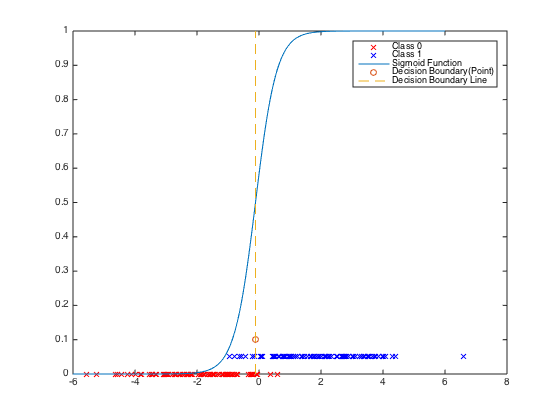
\includegraphics[scale=0.9]{../plot/plot}
\end{document}

